\documentclass{whiteboard}
\begin{document}
\begin{frame}[plain,t]
\bbcover{Grafos}{Ordenação Topológica}{Prof. Edson Alves}{Faculdade UnB Gama}

\end{frame}
\begin{frame}[plain,t]
\begin{tikzpicture}
\node[draw,opacity=0] at (0, 0) {x};
\node[draw,opacity=0] at (14, 8) {x};

	\node[anchor=west] (title) at (0.0, 6.0) { \Large \bbbold{Ordenação topológica} };
\end{tikzpicture}
\end{frame}
\begin{frame}[plain,t]
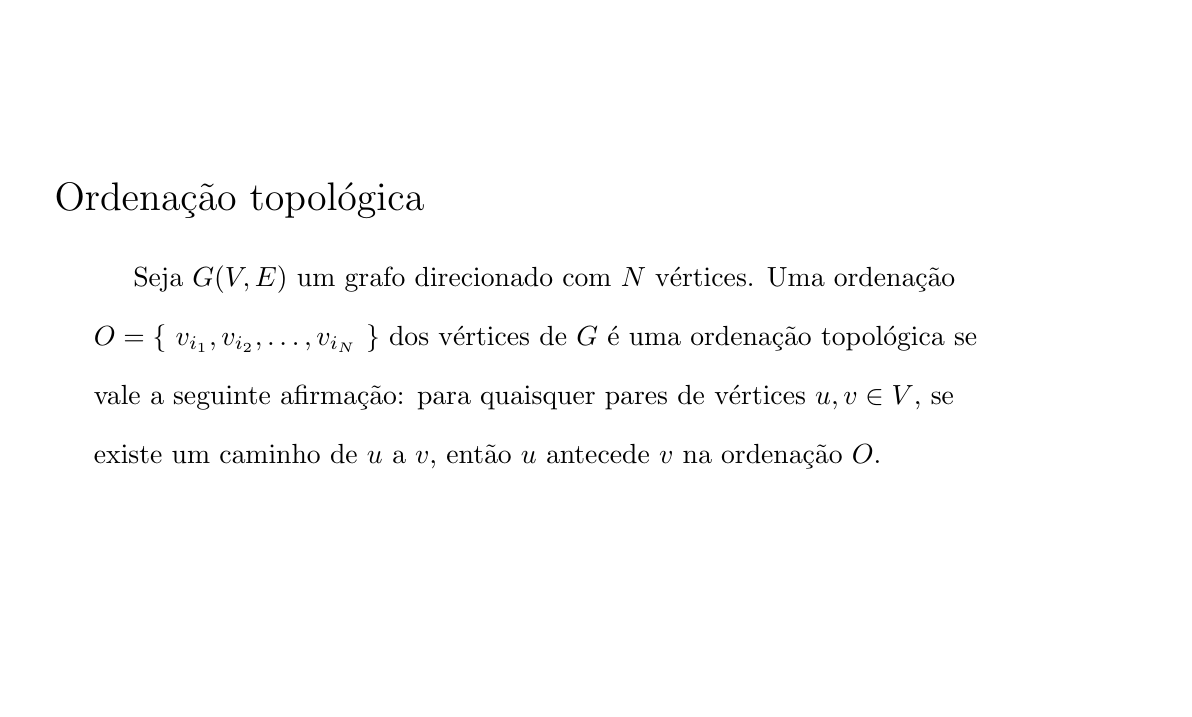
\begin{tikzpicture}
\node[draw,opacity=0] at (0, 0) {x};
\node[draw,opacity=0] at (14, 8) {x};

	\node[anchor=west] (title) at (0.0, 6.0) { \Large \bbbold{Ordenação topológica} };

	\node[anchor=west] (a) at (1.0, 5.0) { \bbtext{Seja $G(V, E)$ um grafo direcionado com $N$ vértices. Uma ordenação } };

	\node[anchor=west] (b) at (0.5, 4.25) { \bbtext{$O = \{\ v_{i_1}, v_{i_2}, \ldots, v_{i_N}\ \}$ dos vértices de $G$ é uma \bbbold{ordenação topológica} se} };

	\node[anchor=west] (c) at (0.5, 3.5) { \bbtext{vale a seguinte afirmação: para quaisquer pares de vértices $u, v \in V$, se } };

	\node[anchor=west] (d) at (0.5, 2.75) { \bbtext{existe um caminho de $u$ a $v$, então $u$ antecede $v$ na ordenação $O$.} };

\end{tikzpicture}
\end{frame}
\begin{frame}[plain,t]
\begin{tikzpicture}
\node[draw,opacity=0] at (0, 0) {x};
\node[draw,opacity=0] at (14, 8) {x};

	\node[anchor=west] (title) at (0.0, 7.0) { \Large \bbbold{Características da ordenação topológica} };
\end{tikzpicture}
\end{frame}
\begin{frame}[plain,t]
\begin{tikzpicture}
\node[draw,opacity=0] at (0, 0) {x};
\node[draw,opacity=0] at (14, 8) {x};

	\node[anchor=west] (title) at (0.0, 7.0) { \Large \bbbold{Características da ordenação topológica} };

	\node[anchor=west] (a) at (1.0, 6.0) { $\star$ \bbtext{Grafos que possuem ciclos não possuem ordenações topológicas} };

\end{tikzpicture}
\end{frame}
\begin{frame}[plain,t]
\begin{tikzpicture}
\node[draw,opacity=0] at (0, 0) {x};
\node[draw,opacity=0] at (14, 8) {x};

	\node[anchor=west] (title) at (0.0, 7.0) { \Large \bbbold{Características da ordenação topológica} };

	\node[anchor=west] (a) at (1.0, 6.0) { $\star$ \bbtext{Grafos que possuem ciclos não possuem ordenações topológicas} };


	\node[anchor=west] (b) at (1.0, 5.0) { $\star$ \bbtext{Um grafo direcionado acíclico (DAG) contém, no mínimo, uma ordenação } };

	\node[anchor=west] (b1) at (0.5, 4.5) { \bbtext{topológica} };

\end{tikzpicture}
\end{frame}
\begin{frame}[plain,t]
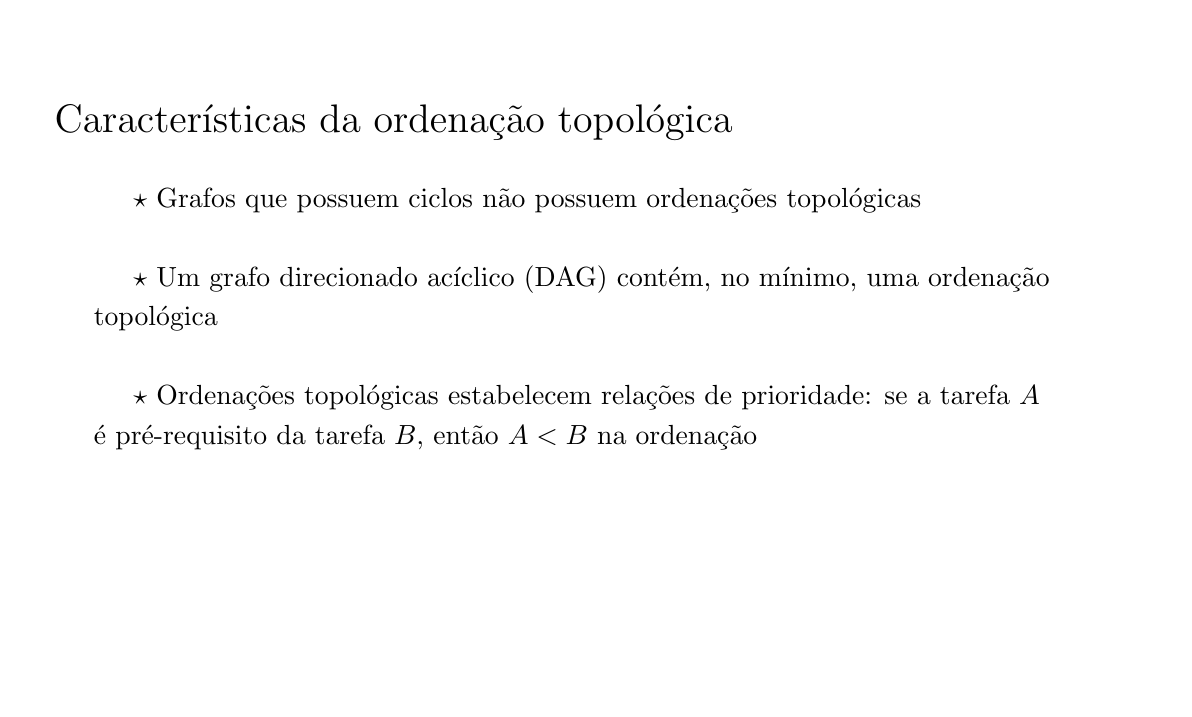
\begin{tikzpicture}
\node[draw,opacity=0] at (0, 0) {x};
\node[draw,opacity=0] at (14, 8) {x};

	\node[anchor=west] (title) at (0.0, 7.0) { \Large \bbbold{Características da ordenação topológica} };

	\node[anchor=west] (a) at (1.0, 6.0) { $\star$ \bbtext{Grafos que possuem ciclos não possuem ordenações topológicas} };


	\node[anchor=west] (b) at (1.0, 5.0) { $\star$ \bbtext{Um grafo direcionado acíclico (DAG) contém, no mínimo, uma ordenação } };

	\node[anchor=west] (b1) at (0.5, 4.5) { \bbtext{topológica} };


	\node[anchor=west] (c) at (1.0, 3.5) { $\star$ \bbtext{Ordenações topológicas estabelecem relações de prioridade: se a tarefa $A$} };

	\node[anchor=west] (c1) at (0.5, 3.0) { \bbtext{é pré-requisito da tarefa $B$, então $A < B$ na ordenação} };

\end{tikzpicture}
\end{frame}
\begin{frame}[plain,t]
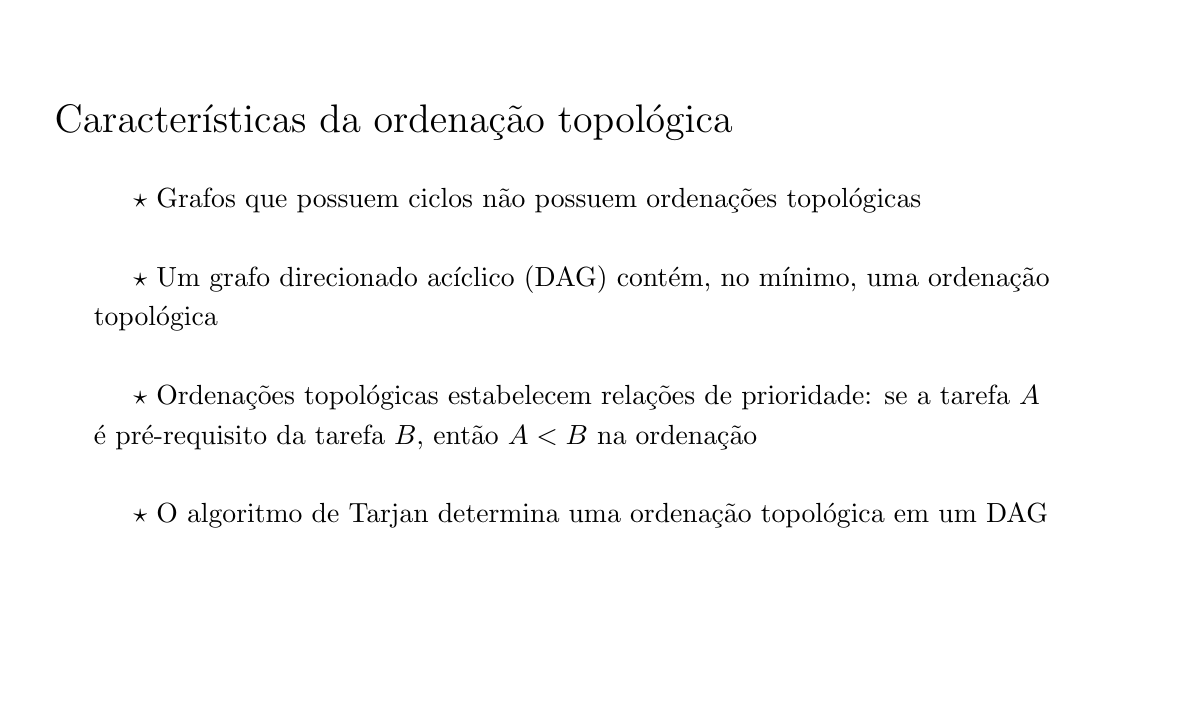
\begin{tikzpicture}
\node[draw,opacity=0] at (0, 0) {x};
\node[draw,opacity=0] at (14, 8) {x};

	\node[anchor=west] (title) at (0.0, 7.0) { \Large \bbbold{Características da ordenação topológica} };

	\node[anchor=west] (a) at (1.0, 6.0) { $\star$ \bbtext{Grafos que possuem ciclos não possuem ordenações topológicas} };


	\node[anchor=west] (b) at (1.0, 5.0) { $\star$ \bbtext{Um grafo direcionado acíclico (DAG) contém, no mínimo, uma ordenação } };

	\node[anchor=west] (b1) at (0.5, 4.5) { \bbtext{topológica} };


	\node[anchor=west] (c) at (1.0, 3.5) { $\star$ \bbtext{Ordenações topológicas estabelecem relações de prioridade: se a tarefa $A$} };

	\node[anchor=west] (c1) at (0.5, 3.0) { \bbtext{é pré-requisito da tarefa $B$, então $A < B$ na ordenação} };


	\node[anchor=west] (d) at (1.0, 2.0) { $\star$ \bbtext{O algoritmo de Tarjan determina uma ordenação topológica em um DAG} };

\end{tikzpicture}
\end{frame}
\begin{frame}[plain,t]
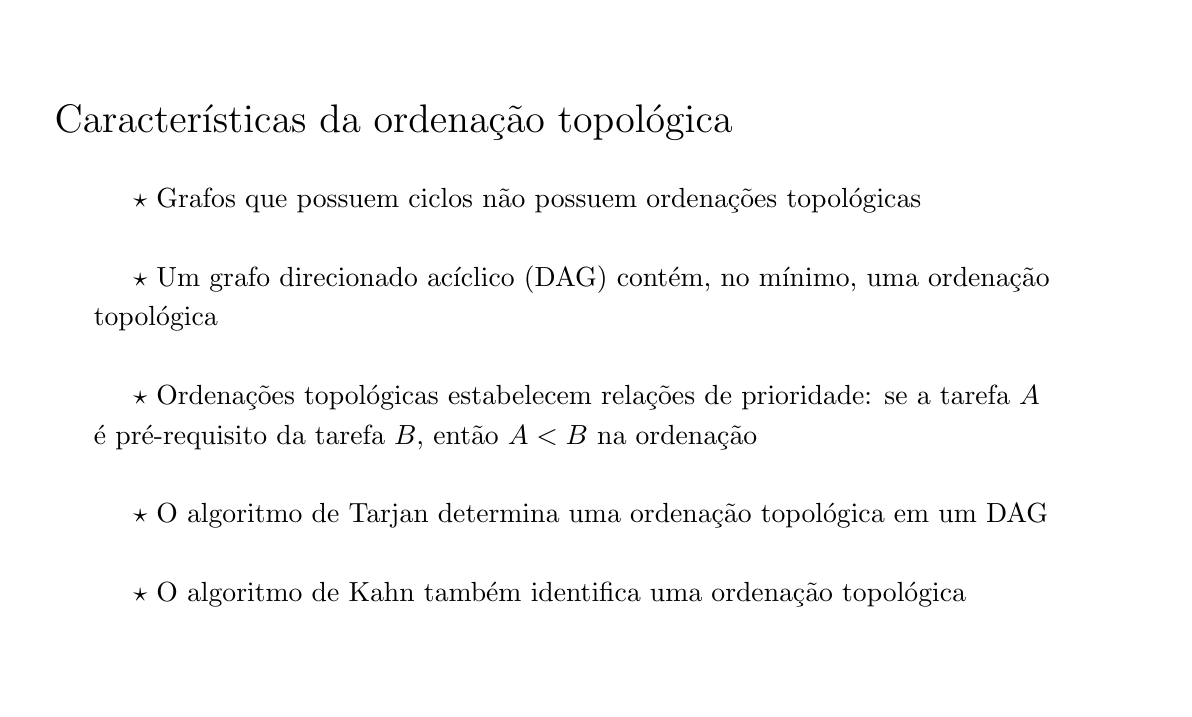
\begin{tikzpicture}
\node[draw,opacity=0] at (0, 0) {x};
\node[draw,opacity=0] at (14, 8) {x};

	\node[anchor=west] (title) at (0.0, 7.0) { \Large \bbbold{Características da ordenação topológica} };

	\node[anchor=west] (a) at (1.0, 6.0) { $\star$ \bbtext{Grafos que possuem ciclos não possuem ordenações topológicas} };


	\node[anchor=west] (b) at (1.0, 5.0) { $\star$ \bbtext{Um grafo direcionado acíclico (DAG) contém, no mínimo, uma ordenação } };

	\node[anchor=west] (b1) at (0.5, 4.5) { \bbtext{topológica} };


	\node[anchor=west] (c) at (1.0, 3.5) { $\star$ \bbtext{Ordenações topológicas estabelecem relações de prioridade: se a tarefa $A$} };

	\node[anchor=west] (c1) at (0.5, 3.0) { \bbtext{é pré-requisito da tarefa $B$, então $A < B$ na ordenação} };


	\node[anchor=west] (d) at (1.0, 2.0) { $\star$ \bbtext{O algoritmo de Tarjan determina uma ordenação topológica em um DAG} };


	\node[anchor=west] (e) at (1.0, 1.0) { $\star$ \bbtext{O algoritmo de Kahn também identifica uma ordenação topológica } };

\end{tikzpicture}
\end{frame}
\begin{frame}[plain,t]
\begin{tikzpicture}
\node[draw,opacity=0] at (0, 0) {x};
\node[draw,opacity=0] at (14, 8) {x};

	\node[anchor=west] (title) at (0.0, 7.0) { \Large \bbbold{Proponente do algoritmo de Tarjan} };

	\node[] (tarjan) at (7.0, 4.0) { \includegraphics[scale=0.12]{figs/tarjan.jpg} };

	\node[] (tname) at (7.0, 1.0) { \bbbold{Robert Endre Tarjan} };

	\node[] (tdate) at (7.0, 0.5) { \bbtext{(1976)} };

\end{tikzpicture}
\end{frame}
\begin{frame}[plain,t]
\begin{tikzpicture}
\node[draw,opacity=0] at (0, 0) {x};
\node[draw,opacity=0] at (14, 8) {x};

	\node[anchor=west] (title) at (0.0, 7.0) { \Large \bbbold{Características do algoritmo de Tarjan} };
\end{tikzpicture}
\end{frame}
\begin{frame}[plain,t]
\begin{tikzpicture}
\node[draw,opacity=0] at (0, 0) {x};
\node[draw,opacity=0] at (14, 8) {x};

	\node[anchor=west] (title) at (0.0, 7.0) { \Large \bbbold{Características do algoritmo de Tarjan} };

	\node[anchor=west] (a) at (1.0, 6.0) { $\star$ \bbtext{O algoritmo de Tarjan determina uma ordenação topológica em um DAG} };

	\node[anchor=west] (a1) at (0.5, 5.5) { \bbtext{por meio de uma DFS modificada} };

\end{tikzpicture}
\end{frame}
\begin{frame}[plain,t]
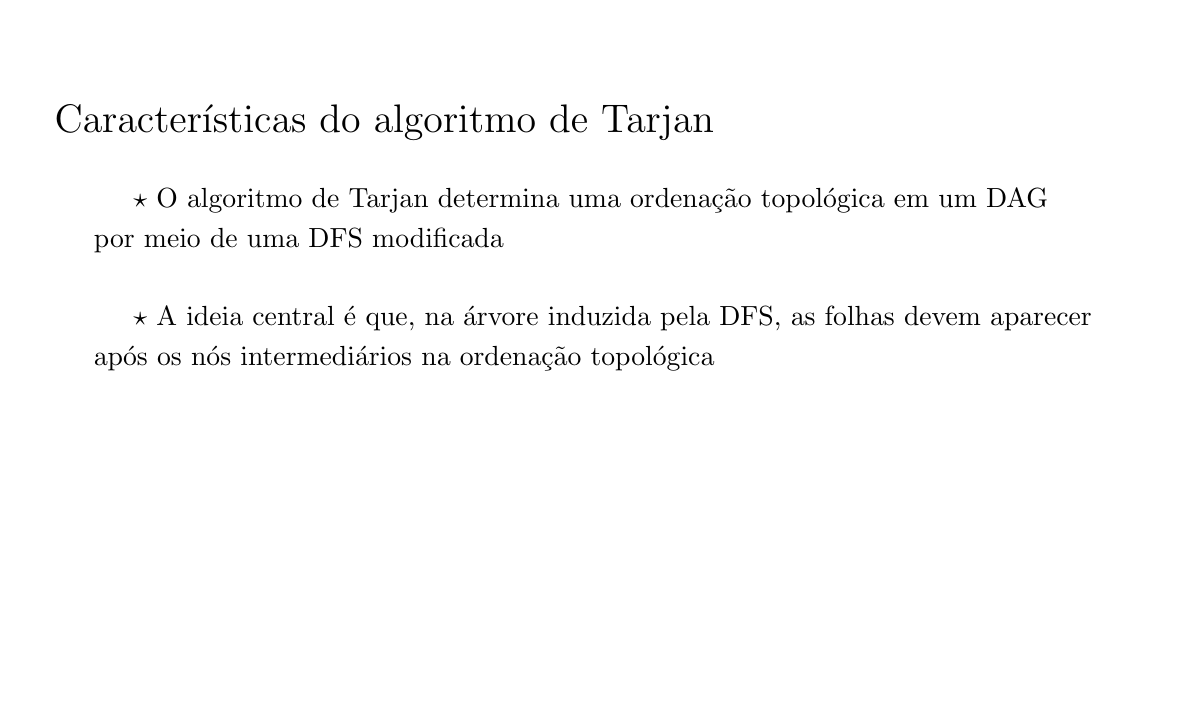
\begin{tikzpicture}
\node[draw,opacity=0] at (0, 0) {x};
\node[draw,opacity=0] at (14, 8) {x};

	\node[anchor=west] (title) at (0.0, 7.0) { \Large \bbbold{Características do algoritmo de Tarjan} };

	\node[anchor=west] (a) at (1.0, 6.0) { $\star$ \bbtext{O algoritmo de Tarjan determina uma ordenação topológica em um DAG} };

	\node[anchor=west] (a1) at (0.5, 5.5) { \bbtext{por meio de uma DFS modificada} };


	\node[anchor=west] (b) at (1.0, 4.5) { $\star$ \bbtext{A ideia central é que, na árvore induzida pela DFS, as folhas devem aparecer} };

	\node[anchor=west] (b1) at (0.5, 4.0) { \bbtext{após os nós intermediários na ordenação topológica} };

\end{tikzpicture}
\end{frame}
\begin{frame}[plain,t]
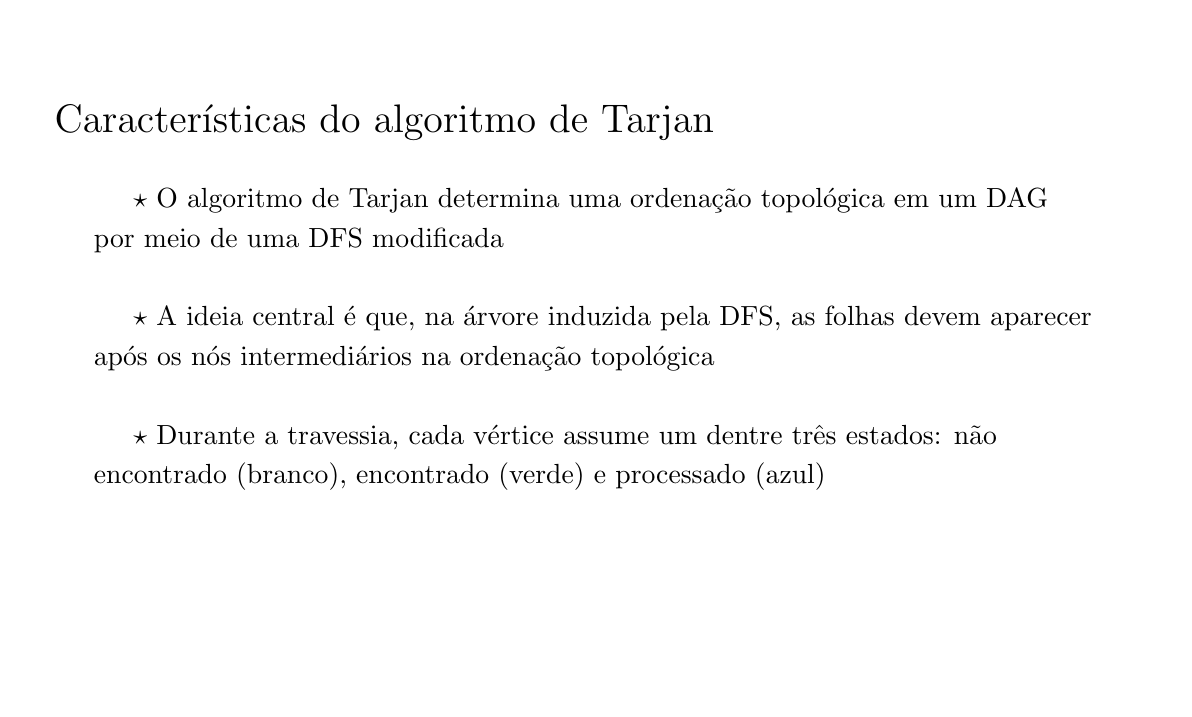
\begin{tikzpicture}
\node[draw,opacity=0] at (0, 0) {x};
\node[draw,opacity=0] at (14, 8) {x};

	\node[anchor=west] (title) at (0.0, 7.0) { \Large \bbbold{Características do algoritmo de Tarjan} };

	\node[anchor=west] (a) at (1.0, 6.0) { $\star$ \bbtext{O algoritmo de Tarjan determina uma ordenação topológica em um DAG} };

	\node[anchor=west] (a1) at (0.5, 5.5) { \bbtext{por meio de uma DFS modificada} };


	\node[anchor=west] (b) at (1.0, 4.5) { $\star$ \bbtext{A ideia central é que, na árvore induzida pela DFS, as folhas devem aparecer} };

	\node[anchor=west] (b1) at (0.5, 4.0) { \bbtext{após os nós intermediários na ordenação topológica} };


	\node[anchor=west] (c) at (1.0, 3.0) { $\star$ \bbtext{Durante a travessia, cada vértice assume um dentre três estados: não} };

	\node[anchor=west] (c1) at (0.5, 2.5) { \bbtext{encontrado (branco), encontrado (verde) e processado (azul)} };

\end{tikzpicture}
\end{frame}
\begin{frame}[plain,t]
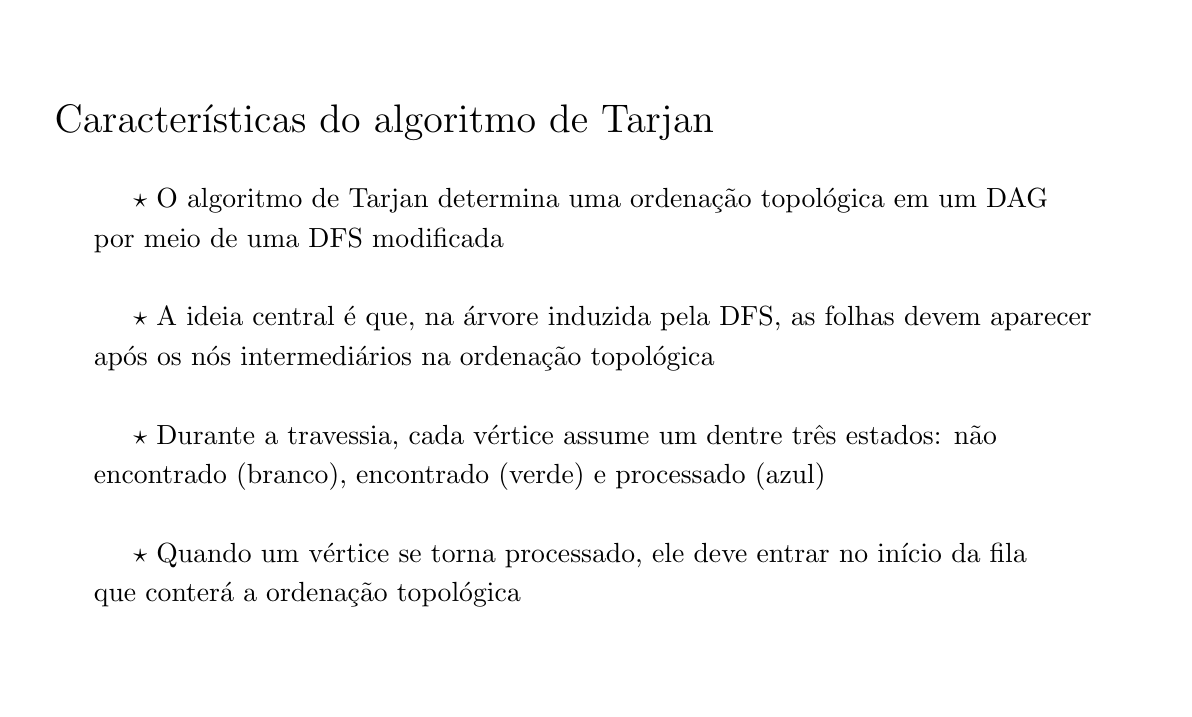
\begin{tikzpicture}
\node[draw,opacity=0] at (0, 0) {x};
\node[draw,opacity=0] at (14, 8) {x};

	\node[anchor=west] (title) at (0.0, 7.0) { \Large \bbbold{Características do algoritmo de Tarjan} };

	\node[anchor=west] (a) at (1.0, 6.0) { $\star$ \bbtext{O algoritmo de Tarjan determina uma ordenação topológica em um DAG} };

	\node[anchor=west] (a1) at (0.5, 5.5) { \bbtext{por meio de uma DFS modificada} };


	\node[anchor=west] (b) at (1.0, 4.5) { $\star$ \bbtext{A ideia central é que, na árvore induzida pela DFS, as folhas devem aparecer} };

	\node[anchor=west] (b1) at (0.5, 4.0) { \bbtext{após os nós intermediários na ordenação topológica} };


	\node[anchor=west] (c) at (1.0, 3.0) { $\star$ \bbtext{Durante a travessia, cada vértice assume um dentre três estados: não} };

	\node[anchor=west] (c1) at (0.5, 2.5) { \bbtext{encontrado (branco), encontrado (verde) e processado (azul)} };


	\node[anchor=west] (d) at (1.0, 1.5) { $\star$ \bbtext{Quando um vértice se torna processado, ele deve entrar no início da fila} };

	\node[anchor=west] (d1) at (0.5, 1.0) { \bbtext{que conterá a ordenação topológica} };

\end{tikzpicture}
\end{frame}
\begin{frame}[plain,t]
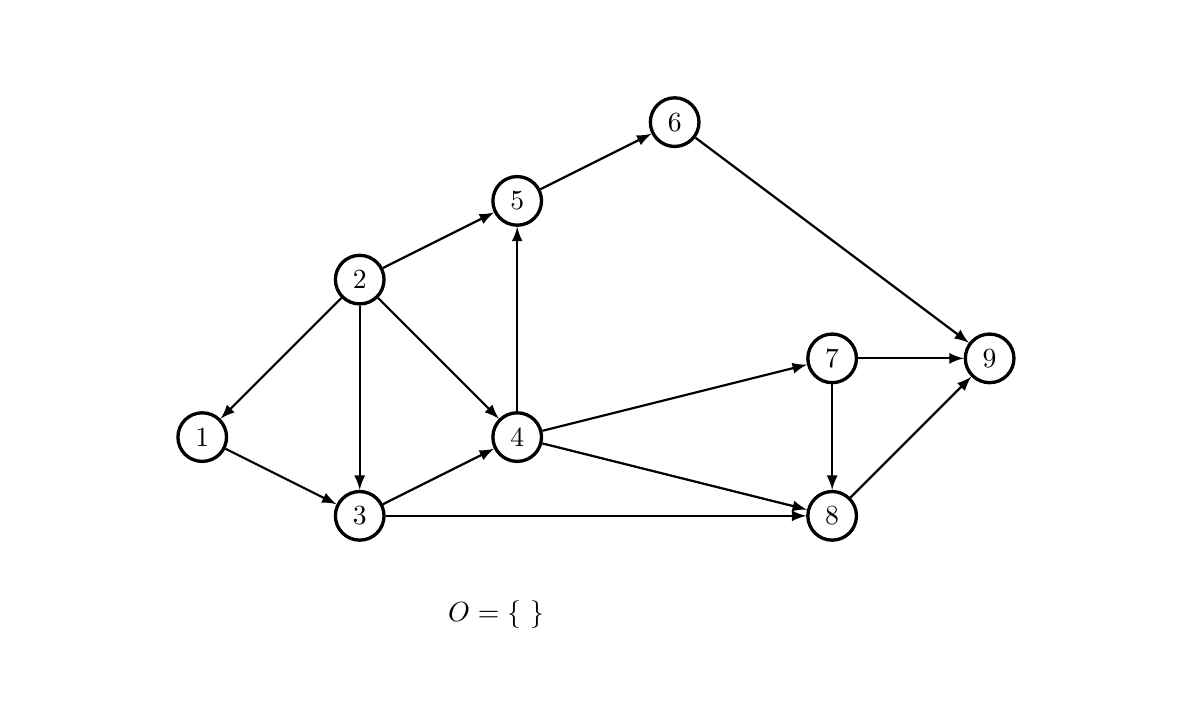
\begin{tikzpicture}
\node[draw,opacity=0] at (0, 0) {x};
\node[draw,opacity=0] at (14, 8) {x};

	\node[very thick,draw,circle] (node1) at (2.0, 3.0) { \bbtext{1} };

	\node[very thick,draw,circle] (node2) at (4.0, 5.0) { \bbtext{2} };

	\node[very thick,draw,circle] (node3) at (4.0, 2.0) { \bbtext{3} };

	\node[very thick,draw,circle] (node4) at (6.0, 3.0) { \bbtext{4} };

	\node[very thick,draw,circle] (node5) at (6.0, 6.0) { \bbtext{5} };

	\node[very thick,draw,circle] (node6) at (8.0, 7.0) { \bbtext{6} };

	\node[very thick,draw,circle] (node7) at (10.0, 4.0) { \bbtext{7} };

	\node[very thick,draw,circle] (node8) at (10.0, 2.0) { \bbtext{8} };

	\node[very thick,draw,circle] (node9) at (12.0, 4.0) { \bbtext{9} };


	\node[anchor=west] (O) at (5.0, 0.75) { \bbtext{$O = \{\ \}$} };

	\draw[thick,-latex](node2) to (node1);

	\draw[thick,-latex](node2) to (node3);

	\draw[thick,-latex](node2) to (node4);

	\draw[thick,-latex](node2) to (node5);

	\draw[thick,-latex](node1) to (node3);

	\draw[thick,-latex](node3) to (node4);

	\draw[thick,-latex](node3) to (node8);

	\draw[thick,-latex](node4) to (node5);

	\draw[thick,-latex](node4) to (node7);

	\draw[thick,-latex](node4) to (node8);

	\draw[thick,-latex](node5) to (node6);

	\draw[thick,-latex](node6) to (node9);

	\draw[thick,-latex](node7) to (node8);

	\draw[thick,-latex](node7) to (node9);

	\draw[thick,-latex](node8) to (node9);





\end{tikzpicture}
\end{frame}
\end{document}
